\documentclass[border=4pt]{standalone}
\usepackage[T1]{fontenc}
\usepackage{mathptmx}
\usepackage{xcolor}
\usepackage{tikz}
\usetikzlibrary{positioning,arrows.meta,calc,fit,backgrounds}
\definecolor{lugar}{HTML}{CDE2FB}
\definecolor{atrator}{HTML}{F6C9B5}
\definecolor{tinta}{HTML}{3B3B38}
\definecolor{azul}{HTML}{2A78D6}
\definecolor{laranja}{HTML}{EB6834}
\begin{document}
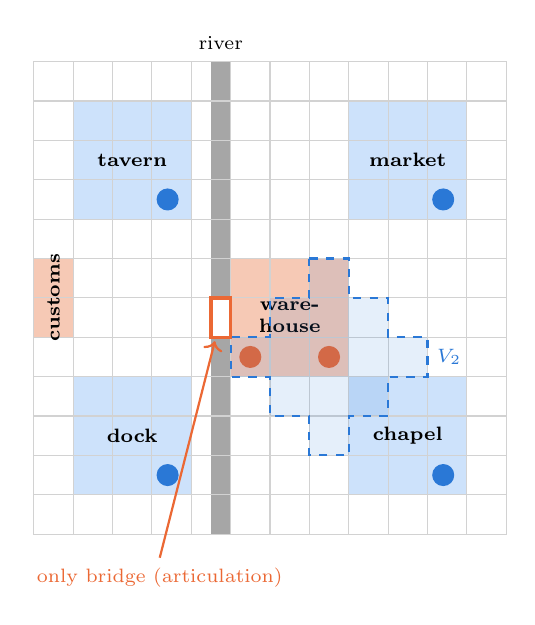
\begin{tikzpicture}[scale=0.5]
  % grade
  \foreach \x in {0,...,11} \foreach \y in {0,...,11} \draw[gray!35] (\x,\y) rectangle ++(1,1);
  % lugares (regiões)
  \newcommand{\regiao}[5]{\fill[#5] (#1,#2) rectangle (#3,#4);}
  \regiao{1}{1}{4}{4}{lugar}     % A
  \regiao{1}{8}{4}{11}{lugar}    % B
  \regiao{5}{4}{8}{7}{atrator}   % C (atrator)
  \regiao{8}{1}{11}{4}{lugar}    % D
  \regiao{8}{8}{11}{11}{lugar}   % E
  \regiao{0}{5}{1}{7}{atrator}   % F
  % barreira (rio) com uma ponte
  \foreach \y in {0,...,11} {\ifnum\y=5\else\fill[gray!70] (4.5,\y) rectangle ++(0.5,1);\fi}
  \foreach \x in {0,...,11} \foreach \y in {0,...,11} \draw[gray!35] (\x,\y) rectangle ++(1,1);
  \node[font=\scriptsize\bfseries] at (2.5,2.5) {dock};
  \node[font=\scriptsize\bfseries] at (2.5,9.5) {tavern};
  \node[font=\scriptsize\bfseries,align=center] at (6.5,5.5) {ware-\\house};
  \node[font=\scriptsize\bfseries] at (9.5,2.5) {chapel};
  \node[font=\scriptsize\bfseries] at (9.5,9.5) {market};
  \node[font=\scriptsize\bfseries,rotate=90] at (0.5,6) {customs};
  % ponte
  \draw[very thick,laranja] (4.5,5) rectangle (5,6);
  \node[font=\scriptsize,anchor=south] at (4.75,12.05) {river};
  \draw[->,laranja,thick] (3.2,-0.6) node[below,font=\scriptsize]{only bridge (articulation)} -- (4.6,4.9);
  % fichas
  \foreach \p/\c in {{3.4,1.5}/azul,{10.4,8.5}/azul,{5.5,4.5}/laranja,{7.5,4.5}/laranja,{10.4,1.5}/azul,{3.4,8.5}/azul}
    \fill[\c] (\p) circle (0.28);
  % raio de percepção de uma ficha (casa da ficha: (7,4))
  \foreach \dx in {-2,...,2} \foreach \dy in {-2,...,2} {
    \pgfmathtruncatemacro{\m}{abs(\dx)+abs(\dy)}
    \ifnum\m<3 \fill[azul,opacity=0.12] (7+\dx,4+\dy) rectangle ++(1,1); \fi}
  \draw[azul,thick,dashed] (7,7)--(8,7)--(8,6)--(9,6)--(9,5)--(10,5)--(10,4)--(9,4)--(9,3)--(8,3)--(8,2)--(7,2)--(7,3)--(6,3)--(6,4)--(5,4)--(5,5)--(6,5)--(6,6)--(7,6)--cycle;
  \node[font=\scriptsize,azul,anchor=west] at (10,4.5) {$V_2$};
\end{tikzpicture}
\end{document}
